\chapter{Introducción a la teoría de grafos}

\label{cap:Intro_Grafos}

Se dice que la Teoría de Grafos tiene su origen en 1736, cuando Euler dio una 
solución al problema (hasta entonces no resuelto) de los siete puentes de 
Königsberg: ¿existe un camino que atraviese cada uno de los puentes exactamente 
una vez?

Para probar que no era posible, Euler sustituyó cada región por un nodo y cada 
puente por una arista, creando el primer grafo que fuera modelo de un problema
matemático. 

\begin{figure}[h]
 \begin{minipage}[b]{.5\textwidth}
  \centering
  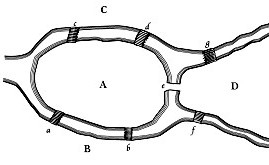
\includegraphics[scale=.75]{fig/images}
  \captionsetup{font=footnotesize}
  \caption{Dibujo de los puentes de Königsberg}
 \end{minipage}
 \begin{minipage}[b]{.5\textwidth}
  \centering
  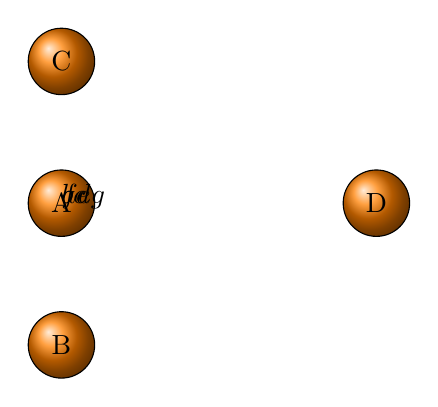
\begin{tikzpicture}
     \GraphInit[vstyle=Shade]
     \begin{scope}
     \tikzstyle{every node} = [draw,
                               shape          = circle,
                               ball color     = orange,
                               text           = black,
                               minimum size   = 24 pt]
     \node (A) at (0,   0){A};
     \node (B) at (0,-1.8){B};
     \node (C) at (0, 1.8){C};
     \node (D) at (4,   0){D};
     \end{scope}
     \begin{scope}
     \tikzset{EdgeStyle/.append style = {bend left}}
     \Edge[label=$b$](A)(B)
     \Edge[label=$c$](A)(C)
     \end{scope}
     \begin{scope}
     \tikzset{EdgeStyle/.append style = {bend right}}
     \Edge[label=$a$](A)(B)
     \Edge[label=$d$](A)(C)
     \end{scope}
     \Edge[label=$f$](B)(D)
     \Edge[label=$e$](A)(D)
     \Edge[label=$g$](C)(D)
  \end{tikzpicture}
  \captionsetup{font=footnotesize}
  \caption{Modelo de los puentes de Königsberg}
 \end{minipage}
\end{figure}

Desde entonces, se ha ido desarrollando esta metodología hasta convertise en
los últimos años en una herramienta importante en áreas del conocimiento muy
variadas como, por ejemplo: la Investigación Operativa, la Computación, la
Ingeniería Eléctrica, la Geografía y la Química. Es por ello que, además, se ha
erigido como una nueva disciplina matemática, que generalmente asociada a las
ramas de Topología y Álgebra.

La utilidad de los grafos se basa en su gran poder de abstracción y una
representación muy clara de cualquier relación, lo que facilita enormemente
tanto la fase de modelado como la de resolución de cualquier problema. Gracias
a la Teoría de Grafos se han desarrollado una gran variedad de algoritmos y
métodos de decisión que podemos implementar a través de lenguajes funcionales y
permiten automatizar la resolución de muchos problemas, a menudo tediosos de
resolver a mano.

\comentario{Pendiente de ampliar la introducción conforme se vaya escribiendo
  los módulos.}

\minitoc

\section{Definición de grafo}

En primer lugar, vamos a introducir terminología básica en el 
desarrollo de la Teoría de Grafos.

\begin{definicion}
  Un \textbf{grafo} $G$ es un par $(V,A)$, donde $V$ es el conjunto 
  cuyos elementos llamamos \textbf{vértices} (o \textbf{nodos}) y 
  $A$ es un conjunto cuyos elementos llamamos \textbf{aristas}. 
\end{definicion}

\begin{definicion}
  Una \textbf{arista} de un grafo $G = (V,A)$, es un conjunto de dos elementos
  de $V$. Es decir, para dos vértices $v,v'$ de $G$, $(v,v')$ y $(v',v)$
  representa la misma arista.
\end{definicion}

\begin{definicion}
  Dado un grafo $G = (V,A)$, diremos que un vértice $v \in V$ es 
  \textbf{adyacente} a $v' \in V$ si $(v',v) \in A$. 
\end{definicion}

\begin{definicion}
  Si en un grafo dirigido se permiten aristas repetidas, lo llamaremos 
  \textbf{multigrafo}. Si no se permiten, lo llamaremos 
  \textbf{grafo regular}.
\end{definicion}

\begin{nota}
  Denotaremos por $|V|$ al número de vértices y por $|A|$ al número de aristas
  del grafo $(V,A)$.
\end{nota}

\begin{ejemplo}
  Sea $G = (V,A)$ un grafo con $V = \{a,b,c,d\}$ y
  $A = \{\allowbreak(a,b), \allowbreak (a,c), \allowbreak (b,d), 
  \allowbreak (d,d)\}$.
  En este grafo, los vértices $a,d$ son adyacentes a $b$.

  \begin{center},
  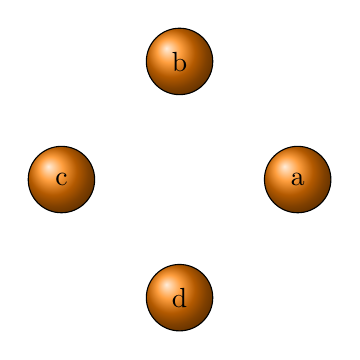
\begin{tikzpicture}
  \SetVertexNoLabel
  \tikzstyle{every node} = [draw, 
                            shape = circle,
                            ball color=orange,
                            minimum size = 24pt]
  \GraphInit [vstyle = Shade]
  \node (a) at (0:1.5){a};
  \node (b) at (90:1.5){b};
  \node (c) at (180:1.5){c};
  \node (d) at (270:1.5){d};
  \Edge (a)(b)
  \Edge (a)(c)
  \Edge (b)(d)
  \Edge (d)(d);
  \end{tikzpicture}
  \end{center}
\end{ejemplo}

\section{El TAD de los grafos}

\label{sec:TAD_grafos}

En esta sección, nos planteamos la tarea de implementar las definiciones
presentadas anteriormente en un lenguaje funcional. En nuestro caso, el
lenguaje que utilizaremos será Haskell. Definiremos el Tipo Abstracto de Dato
(TAD) de los grafos y daremos algunos ejemplos de posibles representaciones de
grafos con las que podremos trabajar.

Si consideramos un grafo finito cualquiera $G = (V,A)$, podemos ordenar el
conjunto de los vértices y representarlo como $V = \{v_1, \dots, v_n\}$ con
$n = |V|$.

En primer lugar, necesitaremos crear un tipo \texttt{(Grafo)} cuya definición
sea compatible con la entidad matemática que representa y que nos permita 
definir las operaciones que necesitamos para trabajar con los grafos. 
Estas operaciones son:

\begin{code}
creaGrafo  -- [a] -> [(a,a)] -> Grafo a
vertices   -- Grafo a -> [a]
adyacentes -- Grafo a -> a -> [a]
aristaEn   -- (a,a) -> Grafo a -> Bool
aristas    -- Grafo a -> [(a,a)]
\end{code}
donde:

\begin{itemize}
\item \texttt{(creaGrafo vs as)} es un grafo tal que el conjunto de sus
  vértices  es \texttt{vs} y el de sus aristas es \texttt{as}.
\item \texttt{(vertices g)} es la lista de todos los vértices del 
  grafo \texttt{g}.
\item \texttt{(adyacentes g v)} es la lista de los vértices adyacentes
  al vértice
  \texttt{v} en el grafo \texttt{g}.
\item \texttt{(aristaEn a g)} se verifica si \texttt{a} es una arista del grafo
  \texttt{g}.
\item \texttt{(aristas g)} es la lista de las aristas del grafo \texttt{g}.
\end{itemize}

\begin{nota}
  Las funciones que aparecen en la especificación del TAD no dependen 
  de la representación que elijamos.
\end{nota}

\begin{ejemplo}

Veamos un ejemplo de creación de grafo y su representación gráfica

\begin{code}
creaGrafo [1..5] [(1,2),(1,3),(1,5),(2,4),
                  (2,5),(3,4),(3,5),(4,5)]
\end{code}

\begin{center}
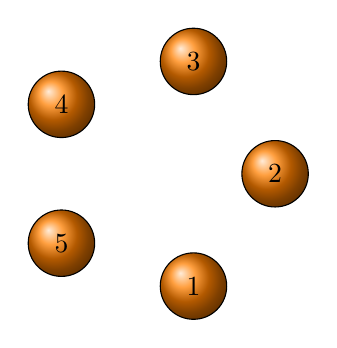
\begin{tikzpicture}
   \tikzstyle{every node} = [draw, 
                             shape        = circle,
                             ball color   = orange,
                             minimum size = 24pt]
   \GraphInit[vstyle=Shade]
   \node (v0) at (4*72:1.5) {1};
   \node (v1) at (   0:1.5) {2};
   \node (v2) at (  72:1.5) {3};
   \node (v3) at (2*72:1.5) {4};
   \node (v4) at (3*72:1.5) {5};
   \Edge(v0)(v1)
   \Edge(v0)(v2)
   \Edge(v0)(v4)
   \Edge(v1)(v3)
   \Edge(v1)(v4)
   \Edge(v2)(v3)
   \Edge(v2)(v4)
   \Edge(v3)(v4);
\end{tikzpicture}
\end{center}
\end{ejemplo}

\subsection{Grafos como listas de aristas}

\entrada{GrafoConListaDeAristas}

\section{Generador de grafos}

\entrada{GeneradorGrafos}

\section{Ejemplos de grafos}

\entrada{EjemplosGrafos}

\section{Definiciones y propiedades}

\entrada{DefinicionesYPropiedades}

\section{Morfismos de grafos}

\entrada{Morfismos}

\section{Conectividad de grafos}

\entrada{ConectividadGrafos}

%%% Local Variables:
%%% mode: latex
%%% TeX-master: "MD_en_Haskell"
%%% End:
